\documentclass[11pt]{article}
\usepackage[margin=2.5cm]{geometry}
\usepackage{amsmath}
\usepackage{booktabs}
\usepackage{graphicx}
\usepackage{parskip}

\title{Cloglog or logit: what each holds constant}
\date{}

\begin{document}
\maketitle

\section*{The difference in one sentence}

The cloglog link assumes that a covariate multiplies the \emph{hazard}, the
risk at each moment for someone still free of plaque, by the same factor
throughout follow-up, so its $e^{\beta}$ is a constant \emph{hazard ratio}.
The logit link assumes that a covariate multiplies the \emph{odds} of having
developed plaque so far by the same factor at every time, so its $e^{\beta}$
is a constant \emph{odds ratio}. Whichever ratio a link holds constant, the
other one has to change as risk builds up.

\section*{The picture}

\begin{center}
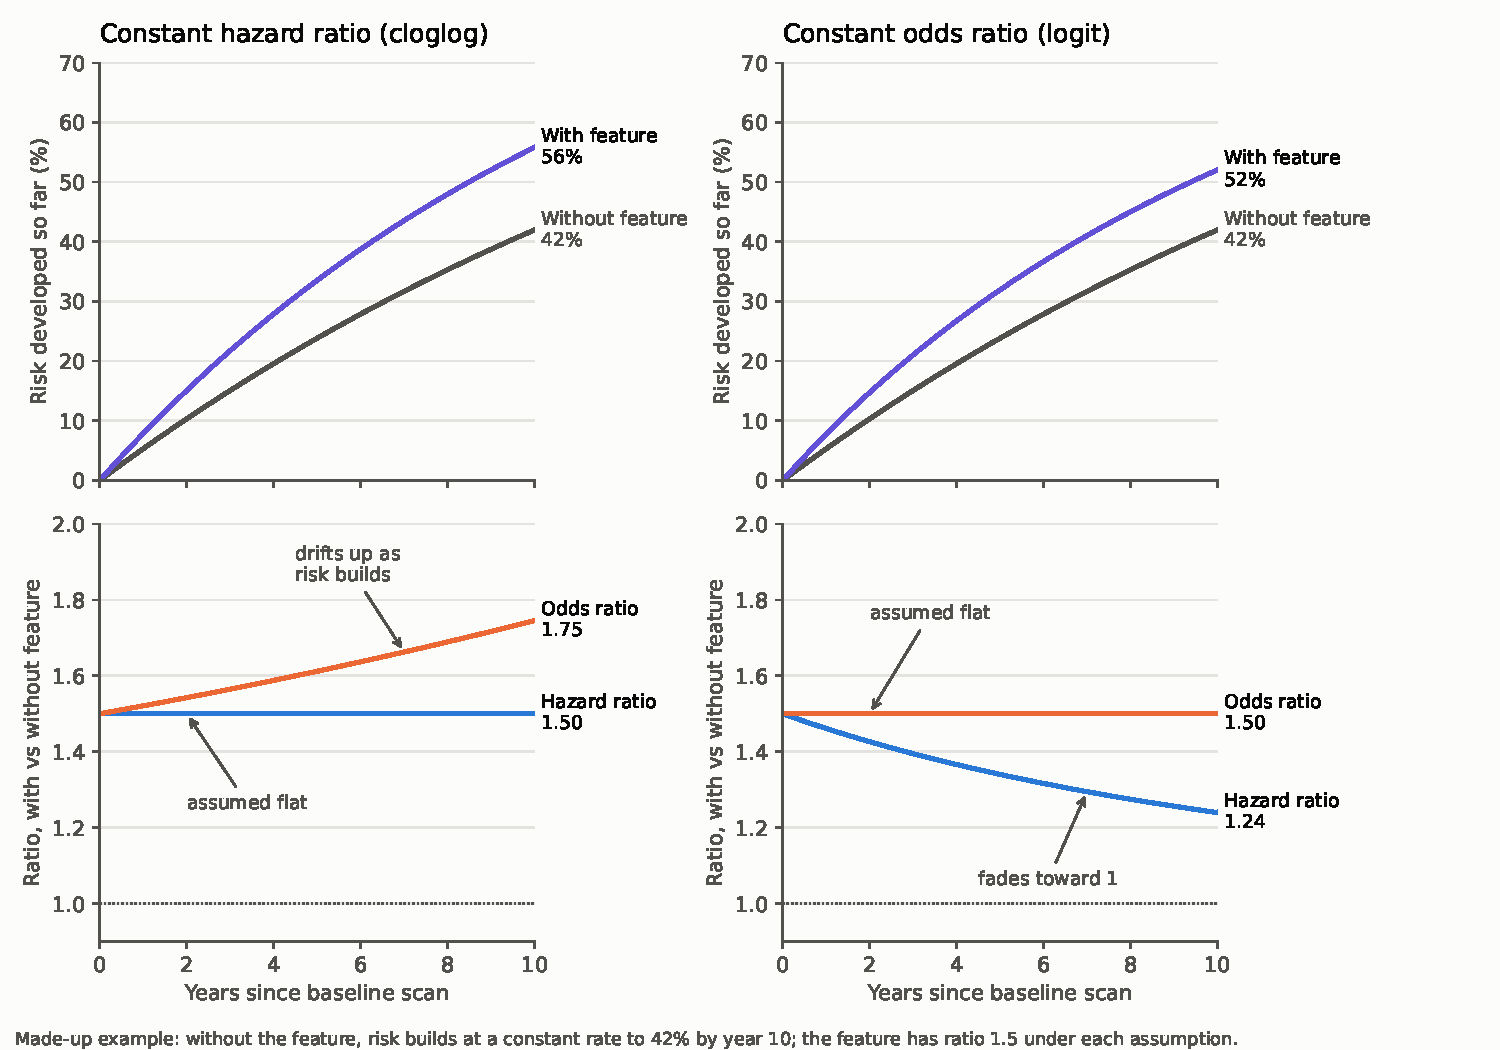
\includegraphics[width=\textwidth]{../hr_vs_or/hr_vs_or.pdf}
\end{center}

The top panels show how much risk each group has built up by each year. The
bottom panels compare the two curves in two ways. The odds ratio compares
the \emph{heights} of the curves at a given year, after turning each height
into odds, $p/(1-p)$. The hazard ratio compares how \emph{steeply} the curves
rise at that year, relative to the people still free of plaque.

On the left (cloglog), the hazard ratio is held at 1.5. The group with the
feature keeps adding risk 1.5 times as fast, and as it pulls ahead its odds
grow faster than its risk, so the odds ratio drifts up to 1.75. On the right
(logit), the odds ratio is held at 1.5. Odds grow faster and faster as risk
rises, so to keep its odds only 1.5 times higher, the group with the feature
has to slow down relative to the other group, and the hazard ratio fades to
1.24. Both ratios start at 1.5: while hardly anyone has plaque, odds and
risks are nearly the same, so the two links nearly agree when the outcome is
rare and part when it is common.

\begin{center}
\begin{tabular}{lll}
\toprule
 & Cloglog & Logit \\
\midrule
Held constant over time & hazard ratio & odds ratio \\
$e^{\beta}$ is & a hazard ratio & an odds ratio \\
The other ratio & odds ratio drifts up & hazard ratio fades toward 1 \\
Scale of the linear predictor & log cumulative hazard & log odds \\
\bottomrule
\end{tabular}
\end{center}

Neither assumption can be checked with one follow-up scan, since the scan
shows whether plaque developed, not when.

\section*{Why cloglog is the smart move in this thesis}

\textbf{The segments add up to a person.} The model is fitted on nine
segments per person, but the question is about people. A person stays free of
plaque only if every segment does. On the hazard scale the segment hazards
simply add, $H_i = \sum_j \Lambda_{ij}$, so the person risk keeps the cloglog
form and needs one integral over the random intercept. Odds do not add, so a
logit model has no such form. This is the reason that decided the choice.

\textbf{It matches how the outcome arises.} Plaque can start at any moment
during follow-up but is only seen at the follow-up scan. The probability of
still being free of plaque is $S = \exp(-H)$, so
$\log\{-\log(1-p)\} = \log H$: the cloglog link is the log cumulative
hazard. Under proportional hazards the log cumulative hazards of two groups
differ by a constant, which is exactly what the linear predictor adds.

\textbf{Follow-up length gets a meaning.} Follow-up varies between people.
Under proportional hazards one hazard ratio holds whatever the length of
follow-up, while an odds ratio would in principle depend on it. Log
follow-up enters the linear predictor with a coefficient $\gamma$, which is
the shape of a Weibull model: $\log H = \text{constant} + \gamma \log t$,
with $\gamma = 1$ a constant hazard and $\gamma > 1$ a rising one.

\textbf{The outcome is common.} About 42\% of people developed plaque. At
that level odds ratios look larger than the change in risk; a hazard ratio
of 1.5 corresponds to an odds ratio of about 1.75.

\textbf{What it does not buy.} At segment level the two links fit about
equally well, and the LR test of the geometry block, the change in C and the
calibration compare fits of the ten-year outcome, whichever ratio is assumed
constant. A logit refit is the planned check that the link does not drive
the results.

\section*{What to cite}

Dobson, A. J. (2002). \emph{An Introduction to Generalized Linear Models},
2nd ed. Chapman \& Hall/CRC. This is the book already cited in the thesis
(\texttt{dobson2002glm}), and it covers every step:

\begin{center}
\begin{tabular}{p{0.45\textwidth}p{0.45\textwidth}}
\toprule
Claim & Dobson (2002) \\
\midrule
$S(y) = \exp[-H(y)]$, $H$ the cumulative hazard & Section 10.2, Eq.~(10.4) \\
Proportional hazards: $h_1 = h_0 e^{x^\top\beta}$, $e^{\beta}$ the hazard ratio, log cumulative hazards differ by a constant & Section 10.2.2, Eqs.~(10.7)--(10.9) \\
$\log H = \log[-\log S]$, the complementary log-log scale; Weibull $\log H = \log\phi + \lambda\log y$ & Section 10.2.3, Eq.~(10.13) \\
The complementary log-log link $\log[-\log(1-\pi)]$ & Section 7.3 \\
Logistic coefficients as log odds ratios & Section 8.3 \\
\bottomrule
\end{tabular}
\end{center}

The step that joins these, that a binary outcome recorded at one follow-up
under proportional hazards gives exactly a cloglog model, is stated as such
in Prentice and Gloeckler (1978), already cited in the thesis as
\texttt{prentice1978grouped} but not yet opened. A textbook that treats
cloglog against logit for events in time intervals is Singer and Willett
(2003), \emph{Applied Longitudinal Data Analysis}, Oxford University Press,
Chapter 12 (not checked).

\end{document}
